\documentclass[11pt,a4paper]{article}

\usepackage{main}
\usepackage{evaluation}

\renewcommand{\typedocument}{Évaluation}
\renewcommand{\classe}{5e}
\renewcommand{\titre}{Interrogation et Rattrapage -- Energie et Electricité}

\begin{document}

\identiteeleve

\creertitre{\titre}

\vspace*{-1em}

\begin{center}
\textit{Durée : 45 minutes -- Calculatrice interdite \\ Tous les exercices sont à faire sur l'énoncé.}
\end{center}

\vspace*{-1em}

\exercice[7]{Questions de cours - Energie}

\question[1.5]{Citer trois formes d'énergie.}

\vspace{0.8em}

\dotfill\par

\question[1.5]{Donner la définition d'une source d'énergie non-renouvelable.}

\vspace{0.8em}

\dotfill\par\vspace{0.8em}

\dotfill\par

\question[1]{Citer deux exemples de sources d'énergie renouvelable.}

\vspace{0.8em}

\dotfill\par

\question[3]{Cocher la ou les bonnes réponses :}

\vspace{0.5em}
\begin{center}
\renewcommand{\arraystretch}{2}
\begin{tabular}{|p{7cm}|c|c|c|}
\hline
Un convertisseur \ldots{} de l'énergie. & $\square$ crée & $\square$ reçoit & $\square$ fournit \\[6pt]
\hline
L'uranium est une source d'énergie \ldots & $\square$ fossile & $\square$ qui émet beaucoup de CO$_2$ & $\square$ non-renouvelable \\[6pt]
\hline
En physique, on peut parler d'énergie \ldots & $\square$ mécanique & $\square$ verte & $\square$ musculaire \\[6pt]
\hline
\end{tabular}
\end{center}

\exercice[3]{Conversion d'énergie}

Dans un jardin, une fontaine à eau est alimentée par un panneau solaire.
Le panneau capte la lumière du soleil et produit de l'électricité, qui alimente une pompe faisant circuler l'eau.
A chaque étape, de l'énergie thermique est perdue.

\question[3]{Compléter la chaîne énergétique ci-dessous en remplaçant les pointillés par les bonnes réponses.}

\begin{center}
    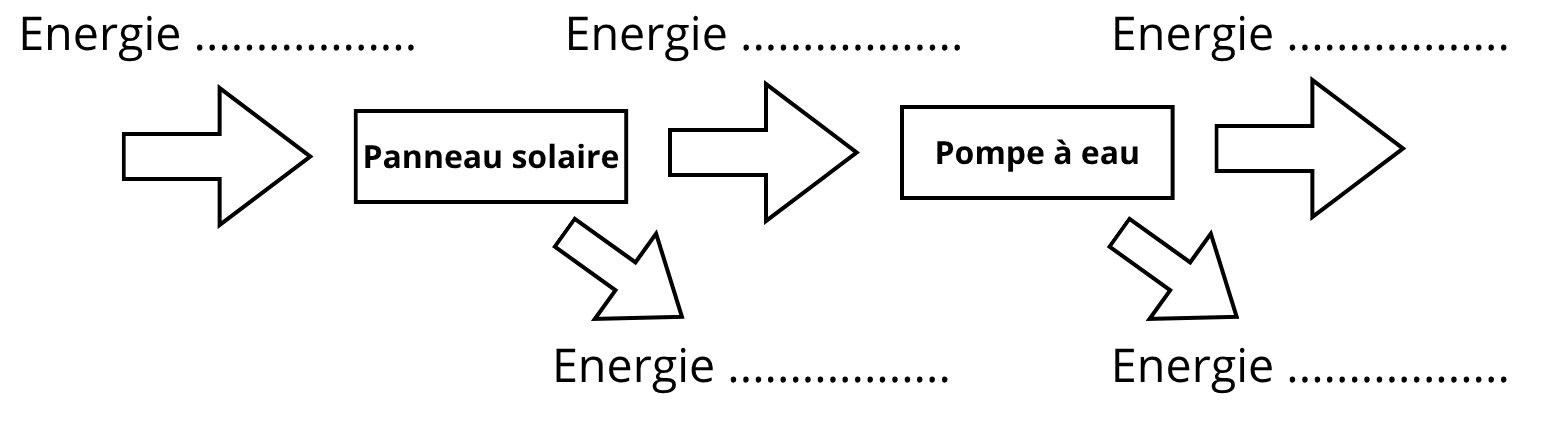
\includegraphics[width=16cm]{images/WE_chaine_energetique.png}
\end{center}

\newpage

\exercice[4]{Questions de cours - Electricité}

\question[2]{Donner la définition d'un court-circuit.}

\vspace{0.8em}

\dotfill\par

\vspace{0.8em}

\dotfill\par

\question[2]{Cocher la ou les bonnes réponses :}

\vspace{0.5em}
\begin{center}
\newcolumntype{C}[1]{>{\centering\arraybackslash}p{#1}}
\renewcommand{\arraystretch}{2}
\begin{tabular}{|C{6.5cm}|C{3.5cm}|C{3.5cm}|C{4.5cm}|}
\hline
Le métal est un matériau \ldots{} & $\square$ conducteur & $\square$ récepteur & $\square$ isolant \\[6pt]
\hline
Un montage en série est constitué \ldots & $\square$ d'une seule boucle & $\square$ de plusieurs boucles & $\square$ de dipôles dont l'ordre \newline n'a pas d'importance \\[6pt]
\hline
\end{tabular}
\end{center}

\exercice[2]{Schémas de dipôles}

Dessiner les symboles des dipôles suivants :

\begin{center}
\renewcommand{\arraystretch}{1}
\newcolumntype{C}[1]{>{\centering\arraybackslash}p{#1}}
\begin{tabular}{|C{4cm}|C{4cm}|C{4cm}|C{4cm}|}
\hline
Lampe & Moteur & Pile & Interrupteur ouvert \\[4pt]
\hline 
 & & & \\[50pt]
\hline
\end{tabular}
\end{center}

\exercice[4]{Circuits électriques}

Indiquer en couleur le passage du courant dans les circuits suivants (colorier les fils) puis entourer les dipôles qui fonctionnent.

\begin{center}
\begin{tabular}{cp{3cm}c}
    
\includegraphics[width=0.2\textwidth]{images/B4a.png} & &
    
\includegraphics[width=0.2\textwidth]{images/B4b.png} \\
    Circuit A & & Circuit B \\
    
\includegraphics[width=0.2\textwidth]{images/4c.png} & &
    
\includegraphics[width=0.25\textwidth]{images/B4d.png} \\
    Circuit C & & Circuit D \\
\end{tabular}
\end{center}

\end{document}